\begin{center}
    \begin{large}
    Cp 2 - Condicionales\\
    Curso \academicyear\\
    \end{large}
    \begin{figure}[h]
    	\centering
    	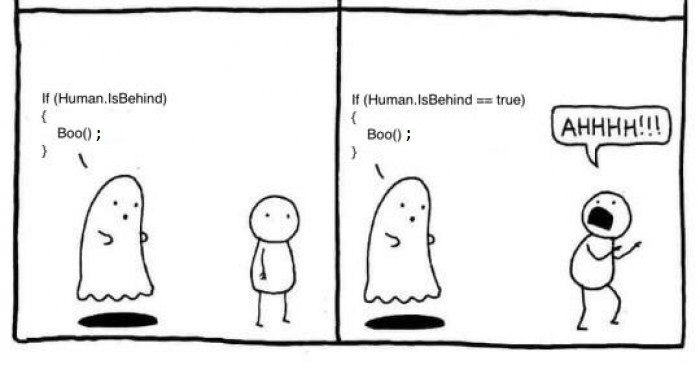
\includegraphics[width=0.6\linewidth]{cp3/conditional.jpg}
    \end{figure}
\end{center}

% Basic 
\section{Número positivo, negativo o cero}
Escribe un programa que lea un número entero y determine si es positivo, negativo o igual a cero.
\subsection*{Ejemplos}
\begin{itemize}
    \item Entrada: \texttt{-5}\\
          Salida: \texttt{El número es negativo.}
    \item Entrada: \texttt{0}\\
          Salida: \texttt{El número es igual a cero.}
    \item Entrada: \texttt{8}\\
          Salida: \texttt{El número es positivo.}
\end{itemize}

\section{Mayor de dos números}
Lee dos números enteros y muestra cuál de ellos es mayor, o indica si son iguales.
\subsection*{Ejemplos}
\begin{itemize}
    \item Entrada: \texttt{12, 7}\\
          Salida: \texttt{El número mayor es 12.}
    \item Entrada: \texttt{4, 9}\\
          Salida: \texttt{El número mayor es 9.}
    \item Entrada: \texttt{10, 10}\\
          Salida: \texttt{Ambos números son iguales.}
\end{itemize}

\section{Par o impar}
Escribe un programa que determine si un número entero no negativo dado es par o impar.
\subsection*{Ejemplos}
\begin{itemize}
    \item Entrada: \texttt{6}\\
          Salida: \texttt{El número es par.}
    \item Entrada: \texttt{13}\\
          Salida: \texttt{El número es impar.}
    \item Entrada: \texttt{0}\\
          Salida: \texttt{El número es par.}
\end{itemize}

\section{Calificación}
Lee una calificación numérica (de 0 a 100) y determina si el estudiante aprobó o reprobó (se aprueba con 60 o más).
\subsection*{Ejemplos}
\begin{itemize}
    \item Entrada: \texttt{75}\\
          Salida: \texttt{El estudiante aprobó.}
    \item Entrada: \texttt{50}\\
          Salida: \texttt{El estudiante reprobó.}
    \item Entrada: \texttt{60}\\
          Salida: \texttt{El estudiante aprobó.}
\end{itemize}

\section{Divisible}
Implemente un programa que reciba dos enteros y determine si el primero es divisible por el segundo.
\subsection*{Ejemplos:}
\begin{itemize}
    \item Entrada: \texttt{10, 2}\\
          Salida: \texttt{10 es divisible por 2.}
    \item Entrada: \texttt{15, 4}\\
          Salida: \texttt{15 no es divisible por 4.}
    \item Entrada: \texttt{20, 5}\\
          Salida: \texttt{20 es divisible por 5.}
    \item Entrada: \texttt{7, 3}\\
          Salida: \texttt{7 no es divisible por 3.}
\end{itemize}

\ifshowanswers
\section*{Respuesta:}
\begin{lstlisting}
Console.WriteLine("Introduce el dividendo:");
int a = int.Parse(Console.ReadLine() ?? string.Empty);
Console.WriteLine("Introduce el divisor:");
int b = int.Parse(Console.ReadLine() ?? string.Empty);

if (b != 0 && a % b == 0)
{
    Console.WriteLine($"{a} es divisible por {b}");
}
else
{
    Console.WriteLine($"{a} no es divisible por {b}");
}
\end{lstlisting}
\fi

\section{Valor absoluto}
Implemente un programa que reciba un número entero \( x \) de la consola y calcule su valor absoluto. El valor absoluto de un número \( x \) se define como el número sin su signo, es decir, la distancia de \( x \) al origen en la recta numérica. No utilice Math.Abs.

La función del valor absoluto \( |x| \) se define de la siguiente manera:
\[
|x| =
\begin{cases} 
x & \text{si } x \geq 0 \\
-x & \text{si } x < 0
\end{cases}
\]

\subsection*{Ejemplos}
\begin{itemize}
    \item Entrada: 5
    
    Salida: El valor absoluto de 5 es: 5

    \item Entrada: -8
    
    Salida: El valor absoluto de -8 es: 8

    \item Entrada: 0
    
    Salida: El valor absoluto de 0 es: 0
\end{itemize}

\ifshowanswers
\section*{Respuesta:}
\begin{lstlisting}
Console.WriteLine("Introduce un número entero:");
int x = int.Parse(Console.ReadLine() ?? string.Empty);
int abs = x >= 0 ? x : -x;
Console.WriteLine($"El valor absoluto de {x} es {abs}");
\end{lstlisting}
\fi

% Intermediate
\section{Mayor de 3}
Implemente un programa que lea tres enteros de la consola e imprima el mayor.
\subsection*{Ejemplos}
\begin{itemize}
    \item Entrada: \texttt{3, 5, 2}\\
          Salida: \texttt{El mayor número es 5.}
    \item Entrada: \texttt{10, 7, 10}\\
          Salida: \texttt{El mayor número es 10.}
    \item Entrada: \texttt{-1, -5, -3}\\
          Salida: \texttt{El mayor número es -1.}
    \item Entrada: \texttt{8, 8, 8}\\
          Salida: \texttt{El mayor número es 8.}
\end{itemize}

\section{Categoría de edad}
Escribe un programa que clasifique a una persona según su edad:
\begin{itemize}
    \item Niño (0-12 años)
    \item Adolescente (13-17 años)
    \item Adulto (18-64 años)
    \item Adulto mayor (65 o más años)
\end{itemize}
\subsection*{Ejemplos}
\begin{itemize}
    \item Entrada: \texttt{7}\\
          Salida: \texttt{Niño}
    \item Entrada: \texttt{15}\\
          Salida: \texttt{Adolescente}
    \item Entrada: \texttt{30}\\
          Salida: \texttt{Adulto}
    \item Entrada: \texttt{65}\\
          Salida: \texttt{Adulto mayor}
\end{itemize}

\section{Triángulo válido}
Dados tres números que representan las longitudes de los lados de un triángulo, determina si forman un triángulo válido. Un triángulo es válido si la suma de las longitudes de dos lados es mayor que la longitud del tercer lado para cualquier combinación de lados.
\subsection*{Ejemplos}
\begin{itemize}
    \item Entrada: \texttt{3, 4, 5}\\
          Salida: \texttt{Triángulo válido}
    \item Entrada: \texttt{1, 2, 3}\\
          Salida: \texttt{No es un triángulo válido}
    \item Entrada: \texttt{6, 8, 10}\\
          Salida: \texttt{Triángulo válido}
\end{itemize}

\section{Número dentro de un rango}
Lee tres números \(a\), \(b\), y \(x\) (donde \(a \leq b\)) y determina si \(x\) se encuentra dentro del rango cerrado \([a, b]\).
\subsection*{Ejemplos}
\begin{itemize}
    \item Entrada: \texttt{2, 8, 5}\\
          Salida: \texttt{Sí, 5 está dentro del rango [2, 8].}
    \item Entrada: \texttt{1, 10, 15}\\
          Salida: \texttt{No, 15 no está dentro del rango [1, 10].}
    \item Entrada: \texttt{3, 9, 9}\\
          Salida: \texttt{Sí, 9 está dentro del rango [3, 9].}
\end{itemize}

\section{Días en un mes}
Escribe un programa que lea un número que representa un mes (1 para enero, 2 para febrero, etc.) y muestre la cantidad de días que tiene ese mes. Considera años no bisiestos, o sea, febrero siempre tendría 28 días.
\subsection*{Ejemplos}
\begin{itemize}
    \item Entrada: \texttt{1}\\
          Salida: \texttt{31 días}
    \item Entrada: \texttt{2}\\
          Salida: \texttt{28 días}
    \item Entrada: \texttt{4}\\
          Salida: \texttt{30 días}
\end{itemize}

\section{Calculadora básica}
Implemente un programa que lea de la consola dos enteros y un operador (+, -, /, *) y realice la operación correspondiente entre ellos e imprima el resultado en consola.
\begin{itemize}
    \item Entrada: \texttt{5, 3, +}\\
    Salida: \texttt{El resultado de 5 + 3 es: 8}
    
    \item Entrada: \texttt{10, 4, -}\\
    Salida: \texttt{El resultado de 10 - 4 es: 6}
    
    \item Entrada: \texttt{8, 7, *}\\
    Salida: \texttt{El resultado de 8 * 7 es: 56}
    
    \item Entrada: \texttt{9, 3, /}\\
    Salida: \texttt{El resultado de 9 / 3 es: 3}
    
    \item Entrada: \texttt{5, 0, /}\\
    Salida: \texttt{Error: División por cero.}
\end{itemize}

% Advanced
\section{Año bisiesto}
Escribe un programa que determine si un año es bisiesto o no. Un año es bisiesto si es divisible entre 4, pero no es divisible entre 100, a menos que también sea divisible entre 400.
\subsection*{Ejemplos}
\begin{itemize}
    \item Entrada: \texttt{2020}\\
          Salida: \texttt{El año 2020 es bisiesto.}
    \item Entrada: \texttt{1900}\\
          Salida: \texttt{El año 1900 no es bisiesto.}
    \item Entrada: \texttt{2000}\\
          Salida: \texttt{El año 2000 es bisiesto.}
\end{itemize}

\section{Cálculo de tarifas}
Escribe un programa que calcule el costo de estacionamiento según el tiempo de permanencia:
\begin{itemize}
    \item Primera hora: \$70
    \item Horas adicionales: \$50 cada una
    \item Máximo diario: \$1000
\end{itemize}
Lee el tiempo de permanencia (en horas) y calcula el costo total.
\subsection*{Ejemplos}
\begin{itemize}
    \item Entrada: \texttt{1}\\
          Salida: \texttt{El costo total es: \$70}
    \item Entrada: \texttt{5}\\
          Salida: \texttt{El costo total es: \$270}
    \item Entrada: \texttt{20}\\
          Salida: \texttt{El costo total es: \$1000}
\end{itemize}

\section{Carnet, de nuevo}
Implemente un programa que le pida al usuario su número de identidad y determine su sexo. El sexo puede determinarse por el penúltimo dígito del número de identidad (par masculino, impar femenino).

\subsection*{Ejemplos}
\begin{itemize}
    \item Entrada: \texttt{02020966175}\\
          Salida: \texttt{Femenino}
    
    \item Entrada: \texttt{04102566345}\\
          Salida: \texttt{Masculino}
    
    \item Entrada: \texttt{05031278457}\\
          Salida: \texttt{Femenino}
\end{itemize}


\ifshowanswers
\section*{Respuesta:}
\begin{lstlisting}
Console.WriteLine("Ingrese su número de identidad:");
long idNumber = long.Parse(Console.ReadLine() ?? string.Empty);
long penultimateDigit = idNumber / 10 % 10;
Console.WriteLine(penultimateDigit % 2 == 0 ? "Masculino" : "Femenino");
\end{lstlisting}
\fi
